\section{Evaluation}
We evaluate our benchmark using a scale 0.1 SolidBench dataset 
(158,233 RDF files, 1,531 vaults, 3,556,159 triples). 
Using the default hyperparameters in Table~\ref{tab:generation_hyperparameters}, 
we generate 8 sequences totaling 192 queries. 
These queries are from the interactive workload, are split into discover and short queries,
with multiple templates belonging to either of these groups.
Experiments run on an Ubuntu 20.04 machine (Intel Core i5-9400) 
with 16 GB RAM allocated to the engine and a 180-second query timeout. 
We repeat each sequence 10 times to minimize variance and 
inject a uniform 70–90 ms latency to simulate a realistic network environment.
The cache is scoped for a sequence, meaning no cache-state is shared between different executions or repetitions of
sequences.

These experiments serve two goals. 
Primarily, we validate the sequence generation by assessing how our three 
design choices impact query correlation, measured via cache \textit{hit rates} and \textit{evictions}. 
Secondarily, we establish a caching performance baseline for a LTQP engine. 
While we report execution speedups to demonstrate the benchmark's utility, 
our focus is on validating the benchmark design rather than exhaustively evaluating the caching algorithms.

% \rt{Can you briefly hint to the subsections that will come hereafter? (so the reader knows what to expect)}

\subsection{Global Cache Performance}

Figure~\ref{fig:global_cache_performance} compares performance profiles~\cite{dolan2002benchmarking} 
for each approach against the no-cache baseline. 
As expected, all caching methods outperform the baseline.

For the unindexed cache, 
small (350k triples) and medium (700k triples) sizes perform similarly. 
The large cache (1,400k triples) significantly improves speed by retaining enough entries across the sequence.
However, the baseline resolves more total queries, 
suggesting cache management overhead causes timeouts for longer queries.

The indexed cache has a higher failure rate, 
as initial indexing costs slow execution when the eviction rate outweighs the increased efficiency of cache hits. 
Still, it accelerates successful queries more than the unindexed cache. 
It also reaches critical capacity sooner, with medium and large sizes performing similarly.

Overall, the indexed cache with cardinality estimation performs best, 
increasing speed and solving more queries. 
Notably, larger cache sizes degrade performance. 
A possible mechanism for this is that the estimator evaluates all cache entries,
including irrelevant unreachable data from past queries. 
This accumulated noise likely can degrade estimates, suggesting the estimator favors smaller, fresher caches.

\begin{figure}[t]
    \centering
    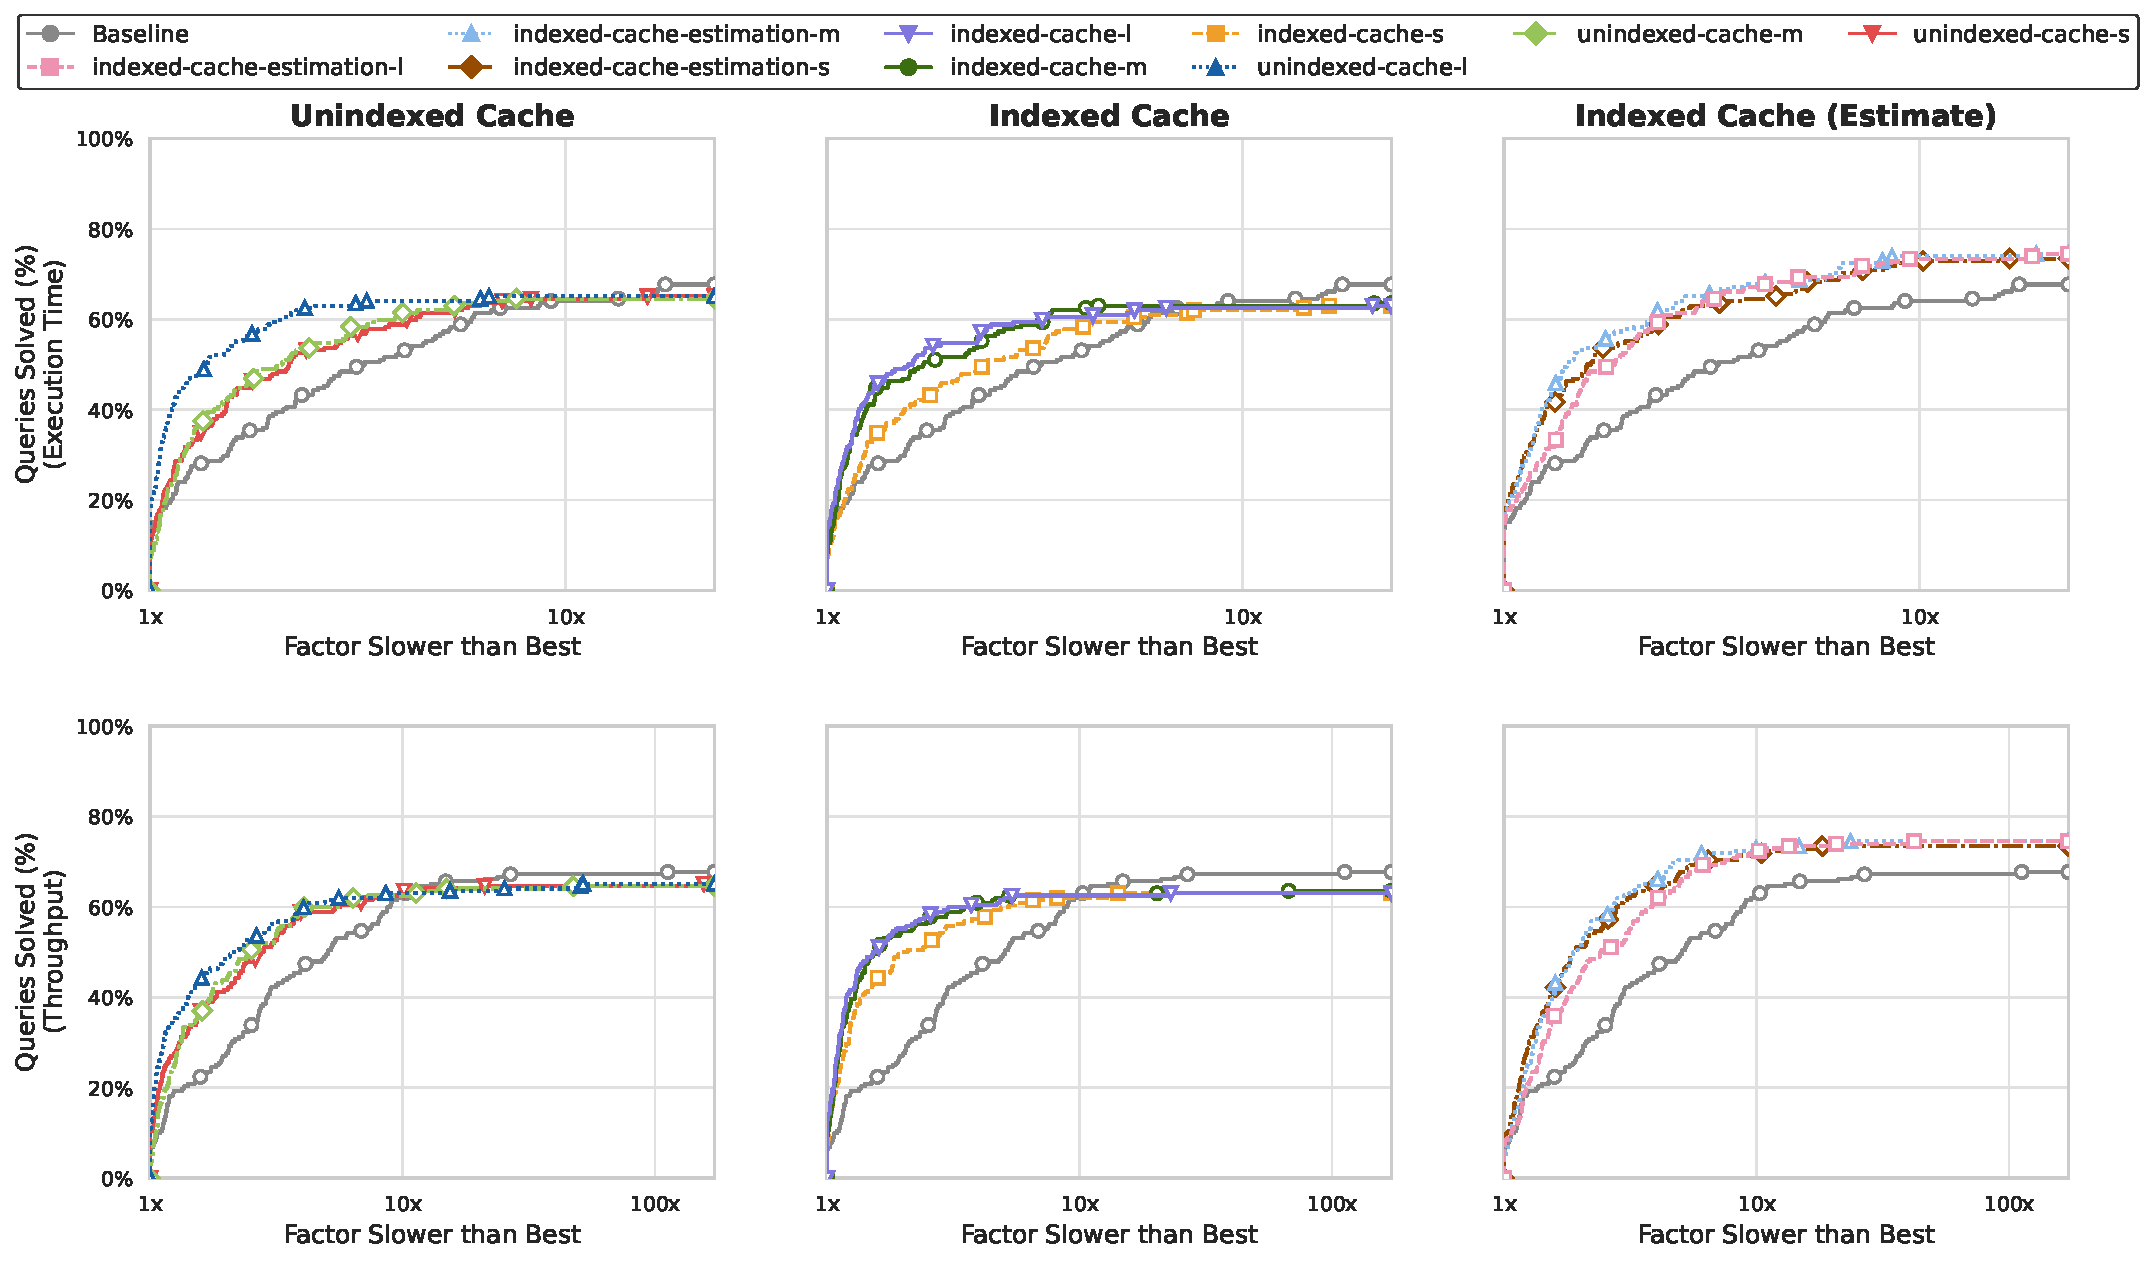
\includegraphics[width=\linewidth]{figures/performance_profile.pdf}
    \caption{Performance profiles of the tested cache algorithms. 
    The y-axis shows the percentage of queries executing within a factor (x-axis) of the fastest algorithm. 
    Curves closer to the top-left indicate better overall performance. 
    The y-intercept ($x=1$) shows how often an algorithm is the outright fastest, 
    while the rightward trajectory demonstrates robustness 
    (e.g., $x=2, y=80\%$ means 80\% of queries execute within twice the fastest time).
    From the figure, we observe that all caching-based approaches outperform the no-cache baseline.}
    \label{fig:global_cache_performance}
\end{figure}

\subsection{Logical Sessions}
To evaluate the impact of logical sessions on caching performance, 
we analyze the hit rate deviation ($\Delta$) from the overall average when queries initiate a new session, 
switch to an existing one, or remain in the current session.
Table~\ref{tab:performance_differences} shows that new sessions severely degrade hit rates,
existing session switches cause moderate degradation, and intra-session queries improve performance.
These effects are strongest in small and medium caches.

Consequently, optimal client-side cache sizing depends heavily on user session-switching behavior.
These findings highlight the need for eviction policies that better retain cross-session entries
and validate our simulation design;
ignoring session dynamics would obscure critical real-world performance shifts.

Future work should investigate whether query sequences should share a frequently accessed core of cache entries.
Protecting these entries from eviction could mitigate the performance penalties of session switching.
Engines could also attempt to identify sessions and keep seperate caches for each session.

\begin{table}[htpb]
\centering
\caption{
    Impact of logical session status on algorithm performance. 
    Values represent absolute and percentage cache hit rate deviations from the global template average across 
    new, existing, and within-session queries. Negative values mean caches perform worse for these types of
    queries.
}
\label{tab:performance_differences}
\begin{tabular*}{\textwidth}{@{\extracolsep{\fill}} l r@{\hspace{1em}}r r@{\hspace{1em}}r r@{\hspace{1em}}r @{}}
\toprule
\textbf{Cache Algorithm} & \multicolumn{2}{c}{\textbf{New Session}} & \multicolumn{2}{c}{\textbf{Existing Session}} & \multicolumn{2}{c}{\textbf{Within Session}} \\
\cmidrule(lr){2-3} \cmidrule(lr){4-5} \cmidrule(lr){6-7}
& \textbf{Abs.} & \textbf{\%} & \textbf{Abs.} & \textbf{\%} & \textbf{Abs.} & \textbf{\%} \\
\midrule
unindexed-l        & -0.066 & -12.278 & -0.014 & -2.474 &  0.011 &  1.931 \\
unindexed-m        & -0.056 & -15.649 & -0.031 & -7.900 &  0.024 &  5.486 \\
unindexed-s        & -0.071 & -24.275 & -0.021 & -6.551 &  0.017 &  4.582 \\
\cmidrule(lr){1-7}
indexed-estimate-l & -0.053 & -10.573 & -0.015 & -2.796 &  0.012 &  2.127 \\
indexed-estimate-m &  0.028 &   7.174 & -0.000 & -0.064 & -0.000 & -0.035 \\
indexed-estimate-s & -0.044 & -14.305 & -0.013 & -3.921 &  0.010 &  2.924 \\
\cmidrule(lr){1-7}
indexed-l          & -0.026 &  -5.011 & -0.003 & -0.571 &  0.003 &  0.467 \\
indexed-m          & -0.087 & -22.782 & -0.021 & -5.098 &  0.017 &  3.682 \\
indexed-s          & -0.033 & -11.036 & -0.015 & -4.470 &  0.012 &  3.153 \\
\bottomrule
\end{tabular*}
\end{table}
\subsection{Refinement Patterns}

To evaluate iterative query refinement simulation, 
we analyze cache behavior across refinement depths. 
Figure 1 shows that hit ratios increase progressively 
as queries undergo sequential refinement. 
Across all algorithms, hit rates increase at depths 2 and 3, 
confirming that refinement heavily reuses prior data.

\begin{figure}[htpb]
    \centering
    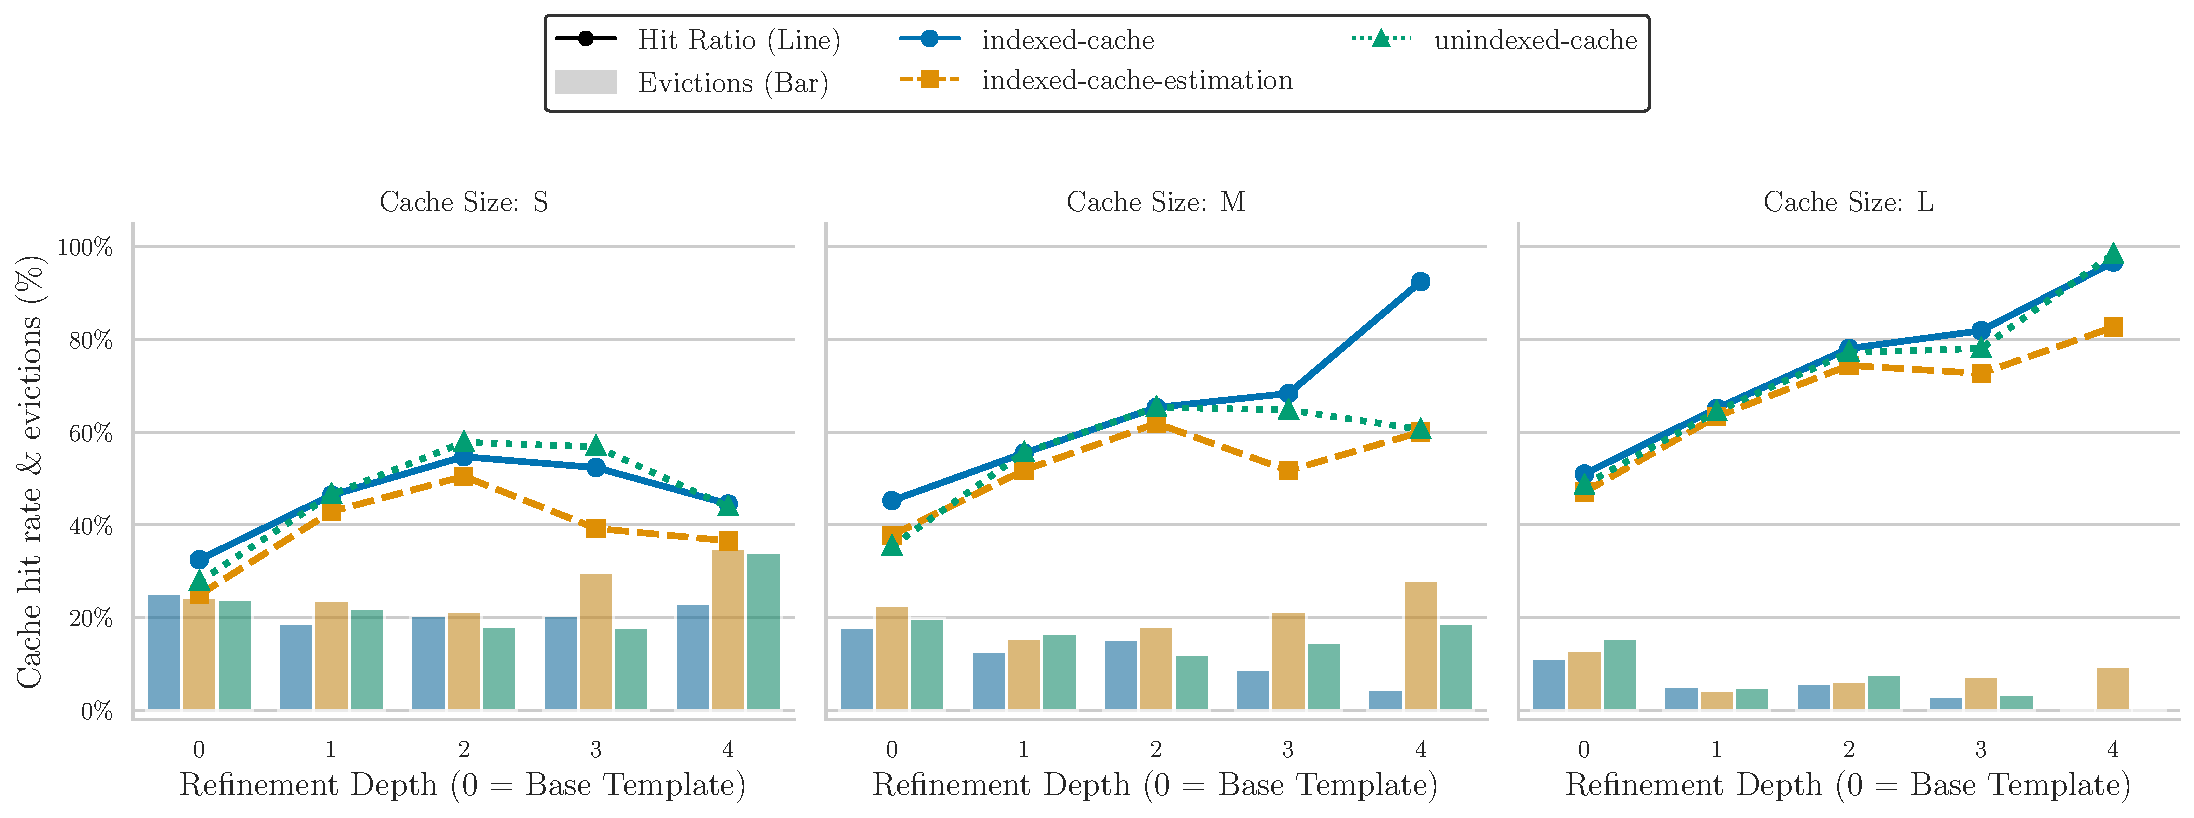
\includegraphics[width=\textwidth]{figures/combined_cache_efficiency.pdf}
    \caption{Cache hit ratios and percentage of cache capacity evicted across refinement depths for small, medium, and large cache configurations.}
    \label{fig:cache_efficiency}
\end{figure}

At higher refinement depths, 
performance depends heavily on cache capacity. 
Large caches sustain high hit rates through depth 4, 
whereas small caches experience significant thrashing,
and degraded hit ratios. 

Surprisingly, the indexed cache without estimation maintains high hit rates at small capacities. 
Different caching mechanisms alter how the Node.js event loop schedules traversal and join executions,
changing traversal order and rate.
We suspect this variance increases temporal locality, though further analysis is needed to confirm the exact mechanism and explain why the indexed cache outperforms the unindexed baseline.

The observed cache hit rate and eviction differences directly translate to measurable execution speedups.
Figure 2 illustrates that the geometric mean speedup generally scales positively with refinement depth, with 
a more pronounced effect for the throughput. 
The indexed-cache algorithm proves particularly effective for prolonged exploratory sequences,
achieving substantial throughput gains at depth 4 compared to the unindexed alternatives.

\begin{figure}[htpb]
    \centering
    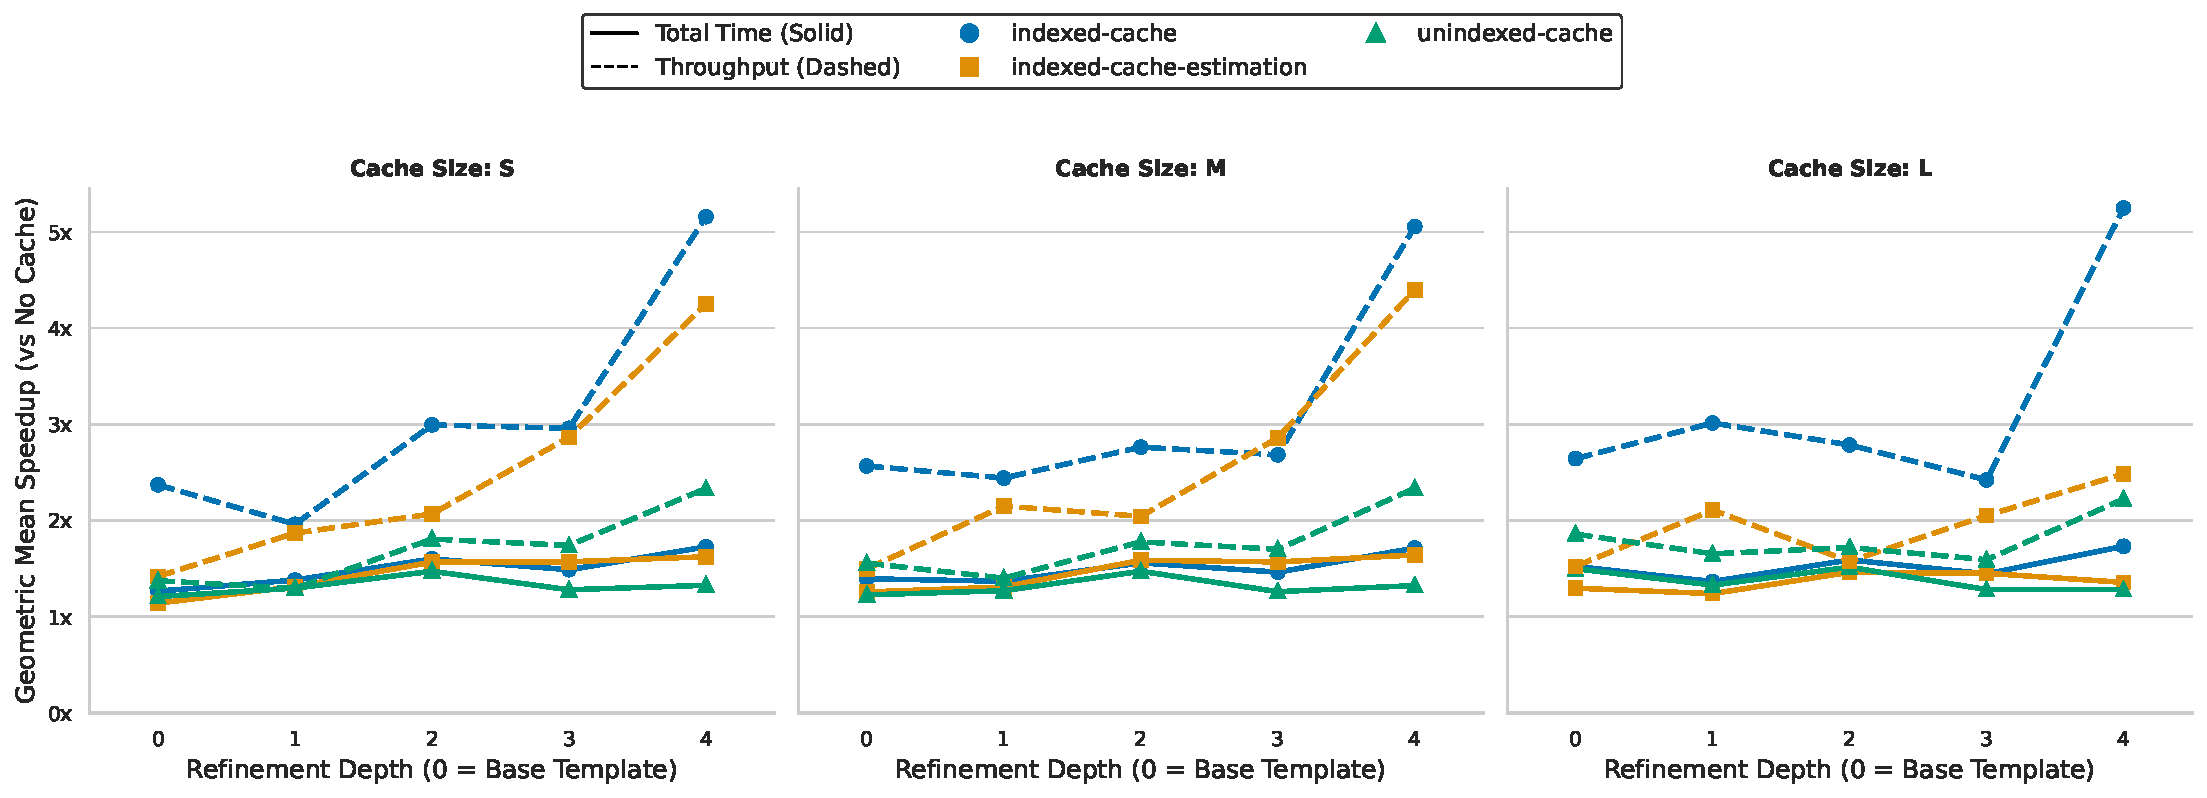
\includegraphics[width=\textwidth]{figures/temporal_throughput_line.pdf}
    \caption{Geometric mean of observed speedups and increases respectively for total execution time and query throughput 
    relative to the no caching baseline across refinement depths.}
    \label{fig:temporal_throughput}
\end{figure}

\subsection{Comparison To Other Evaluation Methods}

\paragraph{Microbenchmarks - Theoretical Hit Rate Analysis}

Cache literature extensively uses microbenchmarks of various forms 
to analyze caching performance~\cite{nicholson2024hpcache,hartig2011caching}.
To compare the conclusions of such a benchmark to the conclusions of the benchmark introduced in this paper
we investigate theoretical caching speedup without management costs, 
by executing each query template twice with simulated cache miss probabilities. 
We excluded the estimation-based approach, 
as using the full cache for estimation would skew the results for miss rates above zero.

Figure~\ref{fig:theoretical_cache_performance} shows representative performance profiles for the workload. 
Most templates (8 out of 12) show reliable improvement that scales with the hit rate for both algorithms. 
However, certain long-running queries (e.g., interactive-discover-6, 7, and short-3) show no speedup, 
and some even experience slowdowns. 
These templates traverse many solid pods but do not require all traversed data. 
We hypothesize that rapidly serving documents from an in-memory cache overwhelms the system with data, 
slowing result production. 
Conversely, HTTP network latency gives the JavaScript event loop time to process the join execution pipeline, 
yielding initial results faster since only the first few requests are needed.

\begin{figure*}[!h]
    \centering
    % Ensure the filename matches your generated PDF
    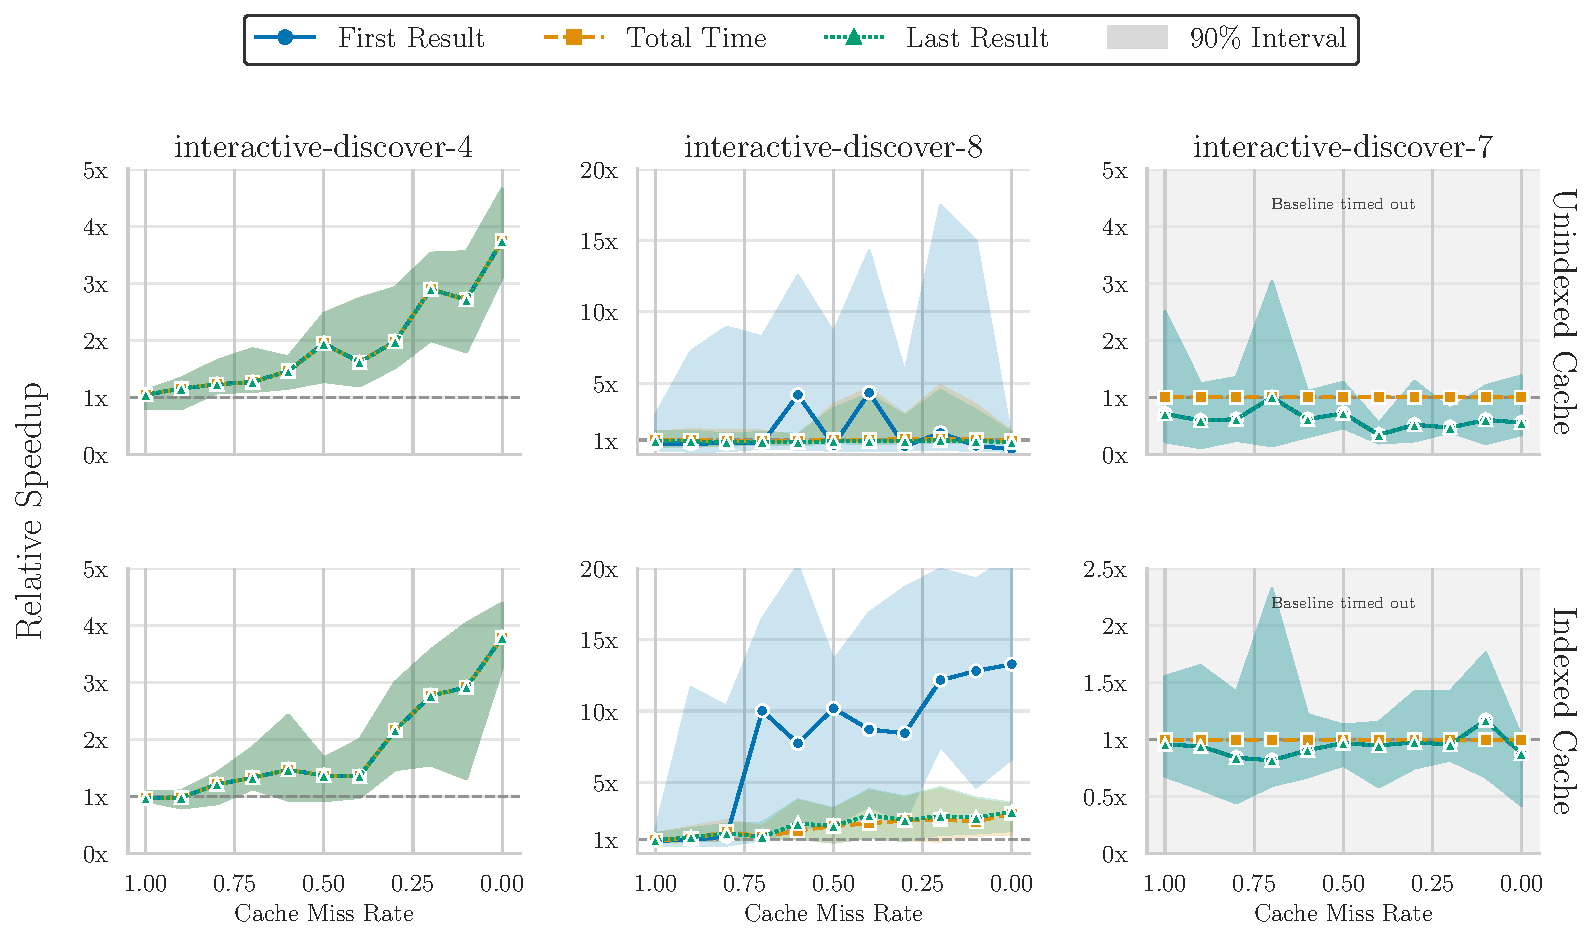
\includegraphics[width=\textwidth]{figures/synth_hit_rate_reduced.pdf}
    \caption{ Performance of unindexed and indexed caches across representative query templates. 
    The y-axis shows the mean speedup relative to a baseline with a 0\% hit rate.
     Shaded regions denote the 90th percentile}
    \label{fig:theoretical_cache_performance}
\end{figure*}

Both caching approaches perform similarly overall, 
but the indexed cache significantly reduces time-to-first-result across most templates. 
As expected, indexed caching is highly advantageous without evictions. 
However, the initial indexing cost creates a trade-off: 
it amplifies both speedups and slowdowns relative to an unindexed cache. 
While this micro-benchmark approach aligns with prior literature~\cite{nicholson2024hpcache}, 
our mixed findings show that micro-benchmarks alone fail to thoroughly evaluate client-side caching optimizations. 
This limitation demonstrates the clear need for the comprehensive benchmark we introduce in this work.




\paragraph{Random Query Sequences}
Another common approach is to use random query sequences from an existing 
benchmark~\cite{o2009star,bizer2011berlin,hartig2011caching,nicholson2024hpcache,folz2016cyclades}.
Figure~\ref{fig:global_cache_performance_random_sequences} shows execution times 
for sequences created by randomly grouping default SolidBench.js queries.
For these random sequences, only large caches perform well,
while smaller ones degrade below the baseline.
These results misleadingly suggest that large caches are vital, 
whereas our benchmark demonstrates significant performance benefits even with smaller sizes.
As expected, the estimation cache performs well in both scenarios because cardinality estimation does not require cache hits.

\begin{figure}[htpb]
    \centering
    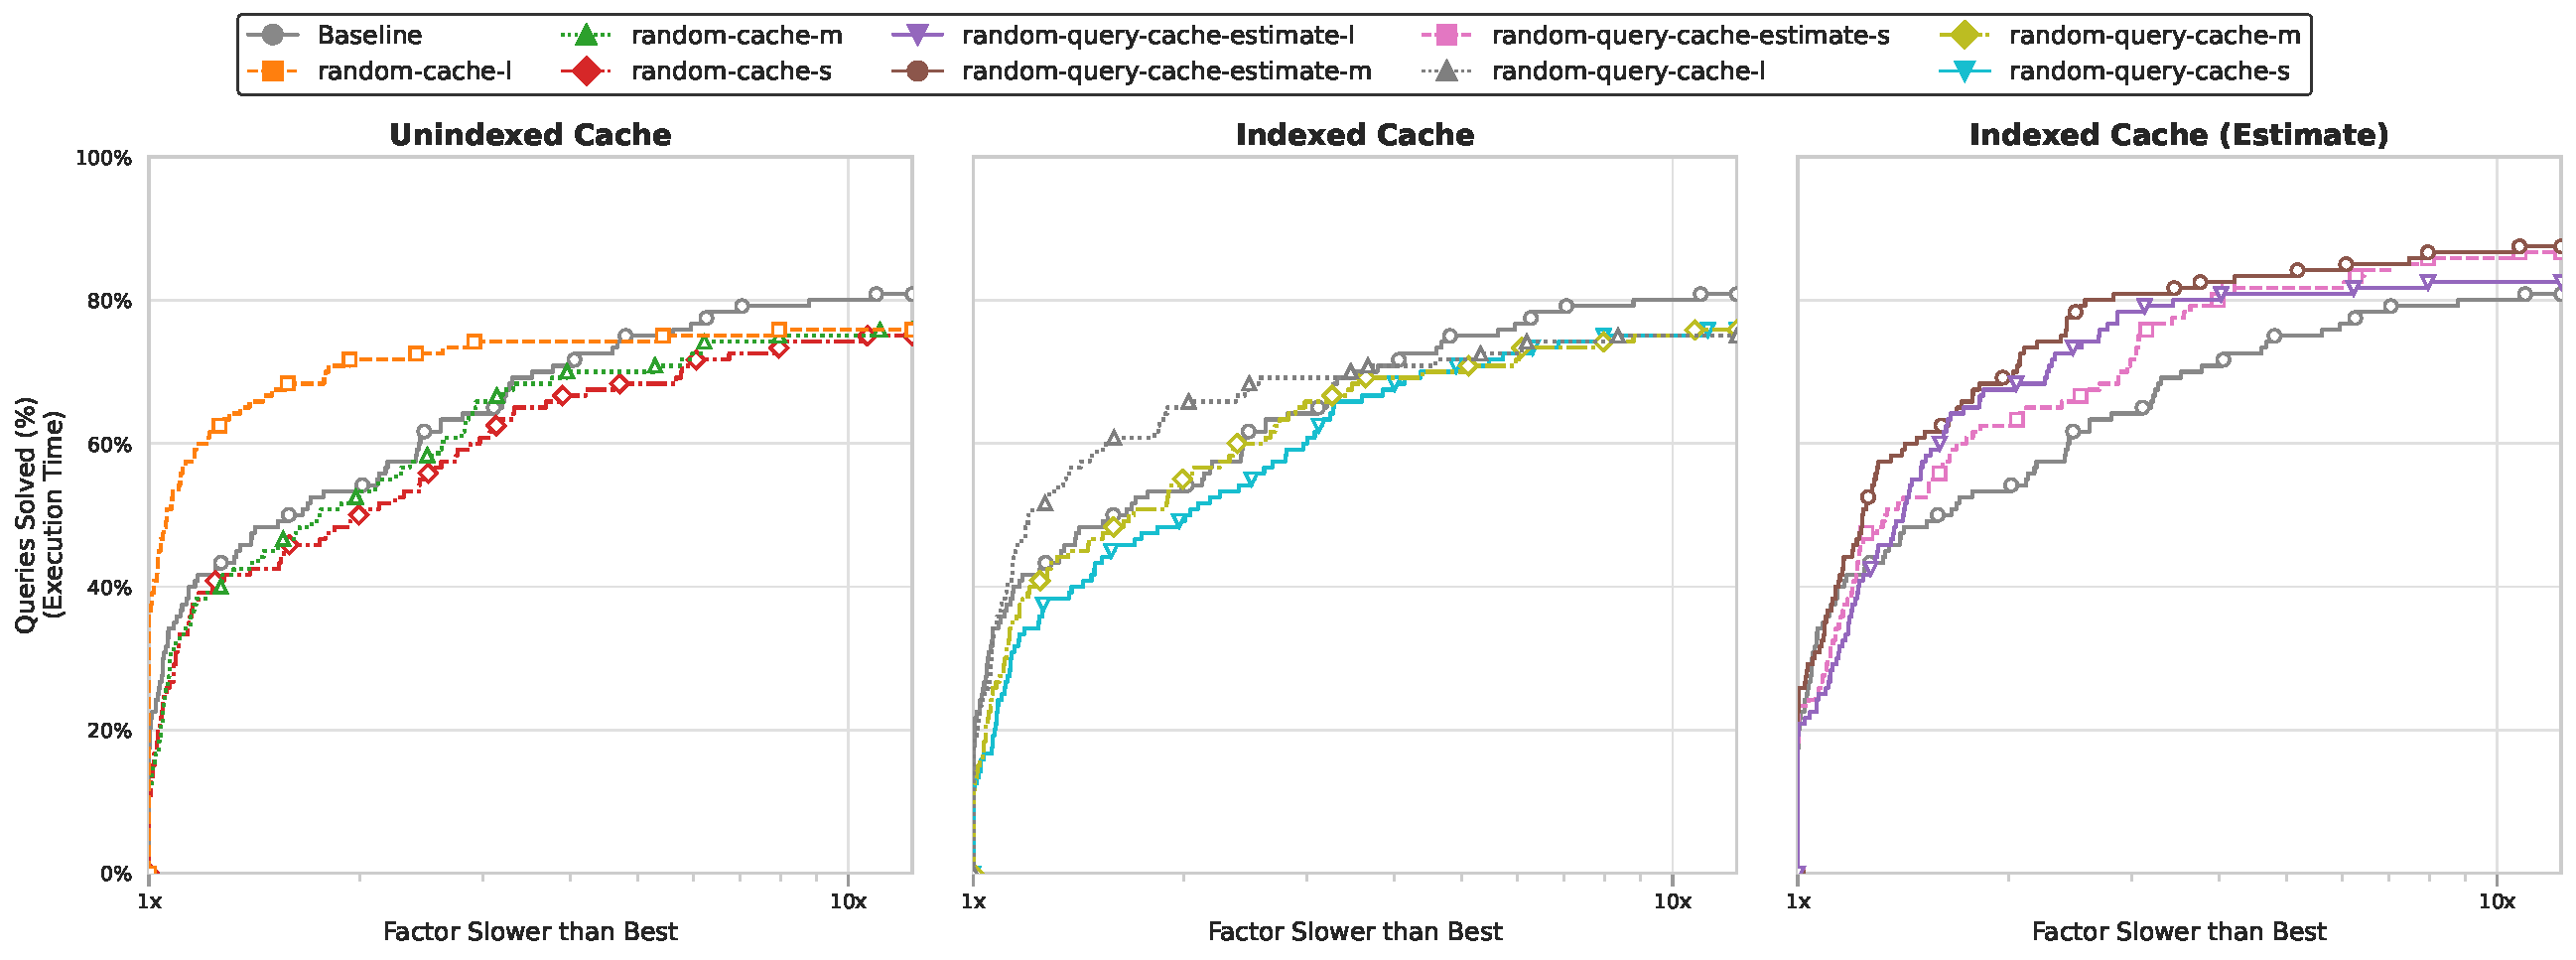
\includegraphics[width=\linewidth]{figures/performance_profile_random_sequences.pdf}
    \caption{Performance profile of the tested cache algorithms on random query sequences.
     The y-axis shows the percentage of queries that execute within 
     a given performance factor (x-axis) of the fastest algorithm for that query.}
    \label{fig:global_cache_performance_random_sequences}
\end{figure}

\paragraph{Scope and Limitations}
We evaluate SolidSessionBench against microbenchmarks and random sequences, 
but explicitly exclude hand-crafted scenarios and simple distributions.
Hand-crafted methods lack scalability, while simple distributions fail to capture complex user habits.
By automating logical sessions and user interests, our benchmark functions as a scalable superset of both approaches,
making direct comparison redundant. 
By contrast, the compared methods do not incorporate these sequence attributes, 
and our results show this omission risks drawing inaccurate conclusions.